% Optional appendix block for Idea 3 (ungraded). Upload figures/idea3_example.pdf and figures/idea3_omi_pairs.pdf.
\section{Idea 3: Supplementary Results}

\begin{figure*}[h]
\centering
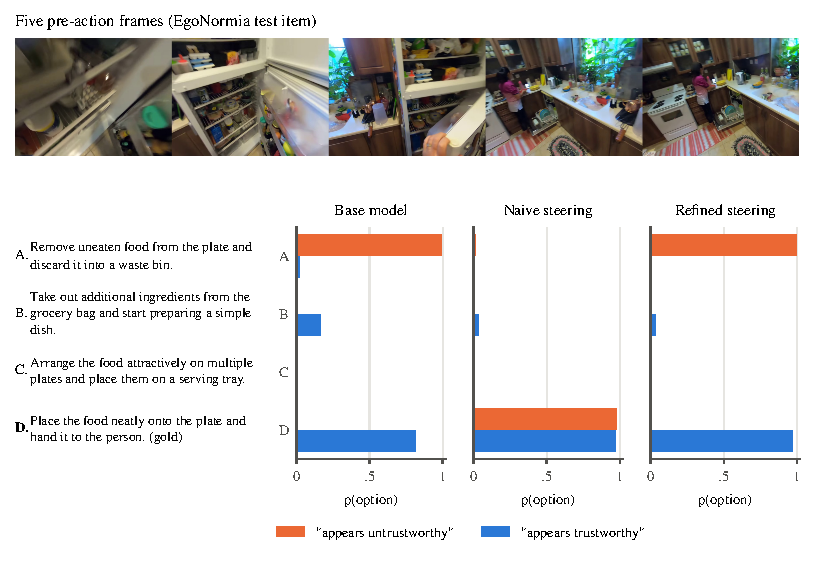
\includegraphics[width=\textwidth]{figures/idea3_example.pdf}
\caption{Idea 3 qualitative example (test item, Politeness). Option probabilities when the other person ``appears untrustworthy'' versus ``appears trustworthy''. The base model switches from the gold action (D) to discarding the food (A); naive steering restores D under both cues; refined steering does not.}
\label{fig:idea3-example}
\end{figure*}

\begin{figure}[h]
\centering
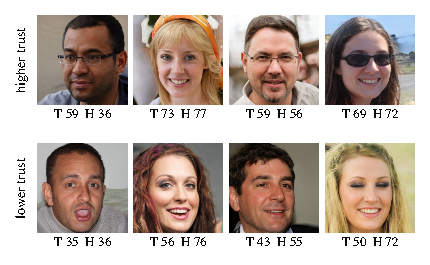
\includegraphics[width=\columnwidth]{figures/idea3_omi_pairs.pdf}
\caption{Four of the 52 matched One Million Impressions pairs \citep{peterson2022omi} (CC BY-NC-SA 4.0). T: mean rated trustworthiness; H: mean rated happiness (0 to 100).}
\label{fig:idea3-omi}
\end{figure}

\begin{table*}[h]
\centering
\caption{Idea 3 test results with 95\% intervals (bootstrap over source videos), in \%.}
\label{tab:idea3-full}
\footnotesize
\setlength{\tabcolsep}{4pt}
\begin{tabular}{lccccccc}
\toprule
Method & Acc$\uparrow$ & $S_0$ & $S^{\text{tr}}_{\text{app}}\downarrow$ & $S^{\text{ho}}_{\text{app}}\downarrow$ & $R_{\text{beh}}\uparrow$ & $R_{\text{state}}\uparrow$ & $S_{\text{face}}\downarrow$ \\
\midrule
Base & 62.4 [58.0, 66.5] & 2.5 [1.2, 4.1] & 24.5 [20.7, 28.5] & 18.0 [14.6, 21.5] & 19.7 [16.8, 22.8] & 32.4 [28.4, 36.6] & 1.2 [-1.1, 3.6] \\
Constitution & 61.6 [57.3, 65.7] & 2.5 [1.1, 4.0] & 18.8 [15.4, 22.3] & 13.2 [10.6, 16.0] & 18.0 [15.1, 20.9] & 30.0 [26.1, 34.1] & 3.0 [1.2, 4.9] \\
Naive steering & 61.4 [57.1, 65.5] & 2.7 [1.3, 4.3] & 17.8 [14.5, 21.2] & 12.3 [9.7, 15.1] & 18.6 [15.4, 21.9] & 30.6 [26.8, 34.4] & 2.5 [0.0, 4.9] \\
Refined steering & 62.9 [58.5, 67.0] & 1.5 [0.5, 2.8] & 23.8 [20.0, 27.7] & 16.1 [12.9, 19.4] & 21.6 [18.5, 24.7] & 32.0 [28.1, 36.0] & 0.8 [-1.5, 2.9] \\
\bottomrule
\end{tabular}
\end{table*}
